% Created by tikzDevice version 0.12.6 on 2024-07-30 09:42:36
% !TEX encoding = UTF-8 Unicode
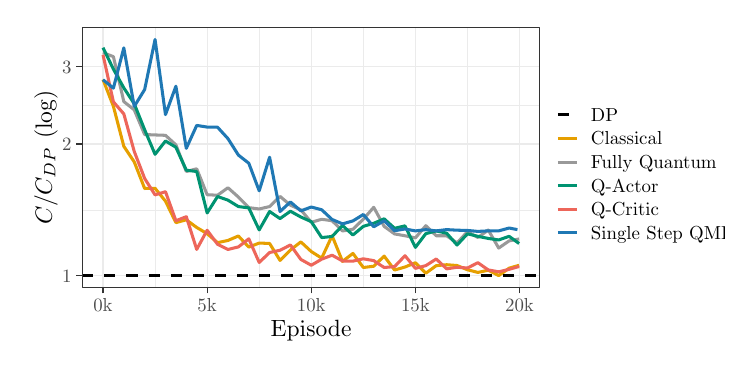
\begin{tikzpicture}[x=1pt,y=1pt]
\definecolor{fillColor}{RGB}{255,255,255}
\path[use as bounding box,fill=fillColor,fill opacity=0.00] (0,0) rectangle (251.96,113.38);
\begin{scope}
\path[clip] (  0.00,  0.00) rectangle (251.96,113.38);
\definecolor{drawColor}{RGB}{255,255,255}
\definecolor{fillColor}{RGB}{255,255,255}

\path[draw=drawColor,line width= 0.4pt,line join=round,line cap=round,fill=fillColor] (  0.00,  0.00) rectangle (251.96,113.38);
\end{scope}
\begin{scope}
\path[clip] ( 19.70, 19.46) rectangle (185.10,113.38);
\definecolor{fillColor}{RGB}{255,255,255}

\path[fill=fillColor] ( 19.70, 19.46) rectangle (185.10,113.38);
\definecolor{drawColor}{gray}{0.92}

\path[draw=drawColor,line width= 0.2pt,line join=round] ( 19.70, 47.54) --
	(185.10, 47.54);

\path[draw=drawColor,line width= 0.2pt,line join=round] ( 19.70, 85.27) --
	(185.10, 85.27);

\path[draw=drawColor,line width= 0.2pt,line join=round] ( 46.03, 19.46) --
	( 46.03,113.38);

\path[draw=drawColor,line width= 0.2pt,line join=round] ( 83.66, 19.46) --
	( 83.66,113.38);

\path[draw=drawColor,line width= 0.2pt,line join=round] (121.29, 19.46) --
	(121.29,113.38);

\path[draw=drawColor,line width= 0.2pt,line join=round] (158.92, 19.46) --
	(158.92,113.38);

\path[draw=drawColor,line width= 0.4pt,line join=round] ( 19.70, 23.73) --
	(185.10, 23.73);

\path[draw=drawColor,line width= 0.4pt,line join=round] ( 19.70, 71.35) --
	(185.10, 71.35);

\path[draw=drawColor,line width= 0.4pt,line join=round] ( 19.70, 99.20) --
	(185.10, 99.20);

\path[draw=drawColor,line width= 0.4pt,line join=round] ( 27.22, 19.46) --
	( 27.22,113.38);

\path[draw=drawColor,line width= 0.4pt,line join=round] ( 64.85, 19.46) --
	( 64.85,113.38);

\path[draw=drawColor,line width= 0.4pt,line join=round] (102.48, 19.46) --
	(102.48,113.38);

\path[draw=drawColor,line width= 0.4pt,line join=round] (140.10, 19.46) --
	(140.10,113.38);

\path[draw=drawColor,line width= 0.4pt,line join=round] (177.73, 19.46) --
	(177.73,113.38);
\definecolor{drawColor}{RGB}{230,159,0}

\path[draw=drawColor,line width= 1.1pt,line join=round] ( 27.22, 94.64) --
	( 30.98, 84.95) --
	( 34.74, 70.51) --
	( 38.51, 64.88) --
	( 42.27, 55.27) --
	( 46.03, 55.34) --
	( 49.80, 50.69) --
	( 53.56, 42.94) --
	( 57.32, 43.95) --
	( 61.08, 41.18) --
	( 64.85, 38.95) --
	( 68.61, 35.69) --
	( 72.37, 36.49) --
	( 76.14, 38.11) --
	( 79.90, 34.09) --
	( 83.66, 35.55) --
	( 87.42, 35.41) --
	( 91.19, 29.27) --
	( 94.95, 33.05) --
	( 98.71, 35.97) --
	(102.48, 32.48) --
	(106.24, 30.10) --
	(110.00, 38.19) --
	(113.76, 28.93) --
	(117.53, 31.81) --
	(121.29, 26.72) --
	(125.05, 27.18) --
	(128.81, 30.84) --
	(132.58, 25.81) --
	(136.34, 26.89) --
	(140.10, 28.43) --
	(143.87, 24.65) --
	(147.63, 27.39) --
	(151.39, 27.72) --
	(155.15, 27.44) --
	(158.92, 25.90) --
	(162.68, 24.94) --
	(166.44, 25.73) --
	(170.21, 23.80) --
	(173.97, 26.47) --
	(177.58, 27.53);
\definecolor{drawColor}{gray}{0.60}

\path[draw=drawColor,line width= 1.1pt,line join=round] ( 27.22,104.36) --
	( 30.98,102.91) --
	( 34.74, 86.68) --
	( 38.51, 83.67) --
	( 42.27, 74.76) --
	( 46.03, 74.62) --
	( 49.80, 74.48) --
	( 53.56, 71.04) --
	( 57.32, 61.41) --
	( 61.08, 62.39) --
	( 64.85, 53.02) --
	( 68.61, 52.83) --
	( 72.37, 55.54) --
	( 76.14, 52.18) --
	( 79.90, 48.35) --
	( 83.66, 47.86) --
	( 87.42, 48.74) --
	( 91.19, 52.41) --
	( 94.95, 49.23) --
	( 98.71, 47.55) --
	(102.48, 43.06) --
	(106.24, 44.14) --
	(110.00, 43.62) --
	(113.76, 39.92) --
	(117.53, 40.54) --
	(121.29, 44.19) --
	(125.05, 48.47) --
	(128.81, 41.58) --
	(132.58, 38.85) --
	(136.34, 38.19) --
	(140.10, 37.42) --
	(143.87, 41.83) --
	(147.63, 38.19) --
	(151.39, 38.19) --
	(155.15, 35.60) --
	(158.92, 39.69) --
	(162.68, 37.57) --
	(166.44, 40.25) --
	(170.21, 33.74) --
	(173.97, 36.34) --
	(177.58, 37.03);
\definecolor{drawColor}{RGB}{0,147,113}

\path[draw=drawColor,line width= 1.1pt,line join=round] ( 27.22,106.16) --
	( 30.98, 98.38) --
	( 34.74, 91.63) --
	( 38.51, 85.87) --
	( 42.27, 76.48) --
	( 46.03, 67.62) --
	( 49.80, 72.44) --
	( 53.56, 70.17) --
	( 57.32, 61.88) --
	( 61.08, 61.40) --
	( 64.85, 46.43) --
	( 68.61, 52.37) --
	( 72.37, 51.06) --
	( 76.14, 48.74) --
	( 79.90, 48.25) --
	( 83.66, 40.30) --
	( 87.42, 46.94) --
	( 91.19, 44.40) --
	( 94.95, 47.05) --
	( 98.71, 44.96) --
	(102.48, 43.29) --
	(106.24, 37.53) --
	(110.00, 37.93) --
	(113.76, 41.90) --
	(117.53, 38.46) --
	(121.29, 41.59) --
	(125.05, 42.70) --
	(128.81, 44.31) --
	(132.58, 40.89) --
	(136.34, 41.76) --
	(140.10, 33.99) --
	(143.87, 38.96) --
	(147.63, 39.92) --
	(151.39, 39.12) --
	(155.15, 34.83) --
	(158.92, 38.89) --
	(162.68, 37.98) --
	(166.44, 37.22) --
	(170.21, 36.68) --
	(173.97, 37.98) --
	(177.58, 35.38);
\definecolor{drawColor}{RGB}{237,102,90}

\path[draw=drawColor,line width= 1.1pt,line join=round] ( 27.22,103.58) --
	( 30.98, 86.57) --
	( 34.74, 82.22) --
	( 38.51, 68.65) --
	( 42.27, 58.89) --
	( 46.03, 52.95) --
	( 49.80, 54.11) --
	( 53.56, 43.61) --
	( 57.32, 45.08) --
	( 61.08, 33.26) --
	( 64.85, 40.18) --
	( 68.61, 35.11) --
	( 72.37, 33.23) --
	( 76.14, 34.16) --
	( 79.90, 37.08) --
	( 83.66, 28.54) --
	( 87.42, 32.13) --
	( 91.19, 32.95) --
	( 94.95, 34.87) --
	( 98.71, 29.63) --
	(102.48, 27.53) --
	(106.24, 29.73) --
	(110.00, 31.16) --
	(113.76, 29.08) --
	(117.53, 29.02) --
	(121.29, 29.86) --
	(125.05, 29.20) --
	(128.81, 26.72) --
	(132.58, 27.04) --
	(136.34, 30.98) --
	(140.10, 26.41) --
	(143.87, 27.39) --
	(147.63, 29.80) --
	(151.39, 26.23) --
	(155.15, 26.81) --
	(158.92, 26.54) --
	(162.68, 28.45) --
	(166.44, 25.84) --
	(170.21, 25.16) --
	(173.97, 26.06) --
	(177.58, 27.08);
\definecolor{drawColor}{RGB}{31,120,180}

\path[draw=drawColor,line width= 1.1pt,line join=round] ( 27.22, 94.55) --
	( 30.98, 91.53) --
	( 34.74,106.07) --
	( 38.51, 84.92) --
	( 42.27, 91.02) --
	( 46.03,109.11) --
	( 49.80, 81.98) --
	( 53.56, 92.22) --
	( 57.32, 69.78) --
	( 61.08, 78.06) --
	( 64.85, 77.46) --
	( 68.61, 77.41) --
	( 72.37, 73.29) --
	( 76.14, 67.34) --
	( 79.90, 64.40) --
	( 83.66, 54.42) --
	( 87.42, 66.56) --
	( 91.19, 46.95) --
	( 94.95, 50.40) --
	( 98.71, 47.18) --
	(102.48, 48.57) --
	(106.24, 47.58) --
	(110.00, 44.07) --
	(113.76, 42.48) --
	(117.53, 43.55) --
	(121.29, 45.87) --
	(125.05, 41.42) --
	(128.81, 43.61) --
	(132.58, 40.02) --
	(136.34, 40.63) --
	(140.10, 39.95) --
	(143.87, 40.39) --
	(147.63, 39.95) --
	(151.39, 40.41) --
	(155.15, 40.20) --
	(158.92, 40.11) --
	(162.68, 39.76) --
	(166.44, 39.96) --
	(170.21, 39.95) --
	(173.97, 40.98) --
	(176.98, 40.41);
\definecolor{drawColor}{RGB}{0,0,0}

\path[draw=drawColor,line width= 1.1pt,dash pattern=on 4pt off 4pt ,line join=round] ( 19.70, 23.73) -- (185.10, 23.73);
\definecolor{drawColor}{gray}{0.20}

\path[draw=drawColor,line width= 0.4pt,line join=round,line cap=round] ( 19.70, 19.46) rectangle (185.10,113.38);
\end{scope}
\begin{scope}
\path[clip] (  0.00,  0.00) rectangle (251.96,113.38);
\definecolor{drawColor}{gray}{0.30}

\node[text=drawColor,anchor=base east,inner sep=0pt, outer sep=0pt, scale=  0.68] at ( 15.88, 21.39) {1};

\node[text=drawColor,anchor=base east,inner sep=0pt, outer sep=0pt, scale=  0.68] at ( 15.88, 69.00) {2};

\node[text=drawColor,anchor=base east,inner sep=0pt, outer sep=0pt, scale=  0.68] at ( 15.88, 96.86) {3};
\end{scope}
\begin{scope}
\path[clip] (  0.00,  0.00) rectangle (251.96,113.38);
\definecolor{drawColor}{gray}{0.20}

\path[draw=drawColor,line width= 0.4pt,line join=round] ( 17.58, 23.73) --
	( 19.70, 23.73);

\path[draw=drawColor,line width= 0.4pt,line join=round] ( 17.58, 71.35) --
	( 19.70, 71.35);

\path[draw=drawColor,line width= 0.4pt,line join=round] ( 17.58, 99.20) --
	( 19.70, 99.20);
\end{scope}
\begin{scope}
\path[clip] (  0.00,  0.00) rectangle (251.96,113.38);
\definecolor{drawColor}{gray}{0.20}

\path[draw=drawColor,line width= 0.4pt,line join=round] ( 27.22, 17.34) --
	( 27.22, 19.46);

\path[draw=drawColor,line width= 0.4pt,line join=round] ( 64.85, 17.34) --
	( 64.85, 19.46);

\path[draw=drawColor,line width= 0.4pt,line join=round] (102.48, 17.34) --
	(102.48, 19.46);

\path[draw=drawColor,line width= 0.4pt,line join=round] (140.10, 17.34) --
	(140.10, 19.46);

\path[draw=drawColor,line width= 0.4pt,line join=round] (177.73, 17.34) --
	(177.73, 19.46);
\end{scope}
\begin{scope}
\path[clip] (  0.00,  0.00) rectangle (251.96,113.38);
\definecolor{drawColor}{gray}{0.30}

\node[text=drawColor,anchor=base,inner sep=0pt, outer sep=0pt, scale=  0.68] at ( 27.22, 10.95) {0k};

\node[text=drawColor,anchor=base,inner sep=0pt, outer sep=0pt, scale=  0.68] at ( 64.85, 10.95) {5k};

\node[text=drawColor,anchor=base,inner sep=0pt, outer sep=0pt, scale=  0.68] at (102.48, 10.95) {10k};

\node[text=drawColor,anchor=base,inner sep=0pt, outer sep=0pt, scale=  0.68] at (140.10, 10.95) {15k};

\node[text=drawColor,anchor=base,inner sep=0pt, outer sep=0pt, scale=  0.68] at (177.73, 10.95) {20k};
\end{scope}
\begin{scope}
\path[clip] (  0.00,  0.00) rectangle (251.96,113.38);
\definecolor{drawColor}{RGB}{0,0,0}

\node[text=drawColor,anchor=base,inner sep=0pt, outer sep=0pt, scale=  0.85] at (102.40,  1.65) {Episode};
\end{scope}
\begin{scope}
\path[clip] (  0.00,  0.00) rectangle (251.96,113.38);
\definecolor{drawColor}{RGB}{0,0,0}

\node[text=drawColor,rotate= 90.00,anchor=base,inner sep=0pt, outer sep=0pt, scale=  0.85] at (  8.70, 66.42) {$C/C_{\text{DP}}$ (log)};
\end{scope}
\begin{scope}
\path[clip] (  0.00,  0.00) rectangle (251.96,113.38);
\definecolor{fillColor}{RGB}{255,255,255}

\path[fill=fillColor] (193.60, 34.94) rectangle (251.96, 97.91);
\end{scope}
\begin{scope}
\path[clip] (  0.00,  0.00) rectangle (251.96,113.38);
\definecolor{fillColor}{RGB}{255,255,255}

\path[fill=fillColor] (190.75, 77.62) rectangle (199.29, 86.15);
\end{scope}
\begin{scope}
\path[clip] (  0.00,  0.00) rectangle (251.96,113.38);
\definecolor{drawColor}{RGB}{0,0,0}

\path[draw=drawColor,line width= 1.1pt,dash pattern=on 4pt off 4pt ,line join=round] (191.61, 81.88) -- (198.44, 81.88);
\end{scope}
\begin{scope}
\path[clip] (  0.00,  0.00) rectangle (251.96,113.38);
\definecolor{fillColor}{RGB}{255,255,255}

\path[fill=fillColor] (190.75, 69.08) rectangle (199.29, 77.62);
\end{scope}
\begin{scope}
\path[clip] (  0.00,  0.00) rectangle (251.96,113.38);
\definecolor{drawColor}{RGB}{230,159,0}

\path[draw=drawColor,line width= 1.1pt,line join=round] (191.61, 73.35) -- (198.44, 73.35);
\end{scope}
\begin{scope}
\path[clip] (  0.00,  0.00) rectangle (251.96,113.38);
\definecolor{fillColor}{RGB}{255,255,255}

\path[fill=fillColor] (190.75, 60.54) rectangle (199.29, 69.08);
\end{scope}
\begin{scope}
\path[clip] (  0.00,  0.00) rectangle (251.96,113.38);
\definecolor{drawColor}{gray}{0.60}

\path[draw=drawColor,line width= 1.1pt,line join=round] (191.61, 64.81) -- (198.44, 64.81);
\end{scope}
\begin{scope}
\path[clip] (  0.00,  0.00) rectangle (251.96,113.38);
\definecolor{fillColor}{RGB}{255,255,255}

\path[fill=fillColor] (190.75, 52.01) rectangle (199.29, 60.54);
\end{scope}
\begin{scope}
\path[clip] (  0.00,  0.00) rectangle (251.96,113.38);
\definecolor{drawColor}{RGB}{0,147,113}

\path[draw=drawColor,line width= 1.1pt,line join=round] (191.61, 56.28) -- (198.44, 56.28);
\end{scope}
\begin{scope}
\path[clip] (  0.00,  0.00) rectangle (251.96,113.38);
\definecolor{fillColor}{RGB}{255,255,255}

\path[fill=fillColor] (190.75, 43.47) rectangle (199.29, 52.01);
\end{scope}
\begin{scope}
\path[clip] (  0.00,  0.00) rectangle (251.96,113.38);
\definecolor{drawColor}{RGB}{237,102,90}

\path[draw=drawColor,line width= 1.1pt,line join=round] (191.61, 47.74) -- (198.44, 47.74);
\end{scope}
\begin{scope}
\path[clip] (  0.00,  0.00) rectangle (251.96,113.38);
\definecolor{fillColor}{RGB}{255,255,255}

\path[fill=fillColor] (190.75, 34.94) rectangle (199.29, 43.47);
\end{scope}
\begin{scope}
\path[clip] (  0.00,  0.00) rectangle (251.96,113.38);
\definecolor{drawColor}{RGB}{31,120,180}

\path[draw=drawColor,line width= 1.1pt,line join=round] (191.61, 39.20) -- (198.44, 39.20);
\end{scope}
\begin{scope}
\path[clip] (  0.00,  0.00) rectangle (251.96,113.38);
\definecolor{drawColor}{RGB}{0,0,0}

\node[text=drawColor,anchor=base west,inner sep=0pt, outer sep=0pt, scale=  0.68] at (203.54, 79.54) {DP};
\end{scope}
\begin{scope}
\path[clip] (  0.00,  0.00) rectangle (251.96,113.38);
\definecolor{drawColor}{RGB}{0,0,0}

\node[text=drawColor,anchor=base west,inner sep=0pt, outer sep=0pt, scale=  0.68] at (203.54, 71.01) {Classical};
\end{scope}
\begin{scope}
\path[clip] (  0.00,  0.00) rectangle (251.96,113.38);
\definecolor{drawColor}{RGB}{0,0,0}

\node[text=drawColor,anchor=base west,inner sep=0pt, outer sep=0pt, scale=  0.68] at (203.54, 62.47) {Fully Quantum};
\end{scope}
\begin{scope}
\path[clip] (  0.00,  0.00) rectangle (251.96,113.38);
\definecolor{drawColor}{RGB}{0,0,0}

\node[text=drawColor,anchor=base west,inner sep=0pt, outer sep=0pt, scale=  0.68] at (203.54, 53.93) {Q-Actor};
\end{scope}
\begin{scope}
\path[clip] (  0.00,  0.00) rectangle (251.96,113.38);
\definecolor{drawColor}{RGB}{0,0,0}

\node[text=drawColor,anchor=base west,inner sep=0pt, outer sep=0pt, scale=  0.68] at (203.54, 45.40) {Q-Critic};
\end{scope}
\begin{scope}
\path[clip] (  0.00,  0.00) rectangle (251.96,113.38);
\definecolor{drawColor}{RGB}{0,0,0}

\node[text=drawColor,anchor=base west,inner sep=0pt, outer sep=0pt, scale=  0.68] at (203.54, 36.86) {Single Step QML};
\end{scope}
\end{tikzpicture}
